

\section{Actividad 3: Característica de salida del JFET}

\subsection{Simulación}

Para la siguiente simulacion vamos a implementar el circuito mostrado en la sección anterior, pero esta vez variamos el voltaje de la fuente $V_{GS}$, y medimos la corriente $I_D$ para distintos valores de $V_{DS}$.

\subsection{Laboratorio}

\paragraph{Instrumental y Materiales}
\begin{itemize}
    \item Multimetro UNI-T UT89X
    \item Transistor JFET MPF102
    \item Resistor de
    \item Fuente de alimentación
\end{itemize}


\begin{table}[ht]
\resizebox{\columnwidth}{!}{%
\begin{tabular}{|l|l|l|}
\hline
\rowcolor[HTML]{FFCC67} 
$V_{DS}$ & $V_{GS} = 172mV$ & $V_{GS} = 250mV$ \\ \hline
1,24V    & 1,56mA           & 0,95mA           \\ \hline
1,6V     & 1,79mA           & 1mA              \\ \hline
2,13V    & 2,05mA           & 1,22mA           \\ \hline
4V       & 2,7mA            & 1,64mA           \\ \hline
6V       & 3,21mA           & 2mA              \\ \hline
10V      & 4mA              & 2,7mA            \\ \hline
15V      & 5,1mA            & 3,52mA           \\ \hline
\end{tabular}%
}
\end{table}

\begin{table}[ht]
\resizebox{\columnwidth}{!}{%
\begin{tabular}{|l|l|l|}
\hline
\rowcolor[HTML]{FFCC67} 
$V_{DS}$ & $V_{GS} = 390mV$ & $V_{GS} = 530mV$ \\ \hline
1,24V    & 0,16mA           & $4,84 \mu A$     \\ \hline
1,6V     & 0,19mA           & $6,28 \mu A$     \\ \hline
2,13V    & 0,24mA           & $8,17 \mu A$     \\ \hline
4V       & 0,39mA           & $16,05 \mu A$    \\ \hline
6V       & 0,55mA           & $25,4 \mu A$     \\ \hline
10V      & 0,9mA            & 0,12mA           \\ \hline
15V      & 1,4mA            & 0,27mA           \\ \hline
\end{tabular}%
}
\end{table}

\vspace{0.1cm}

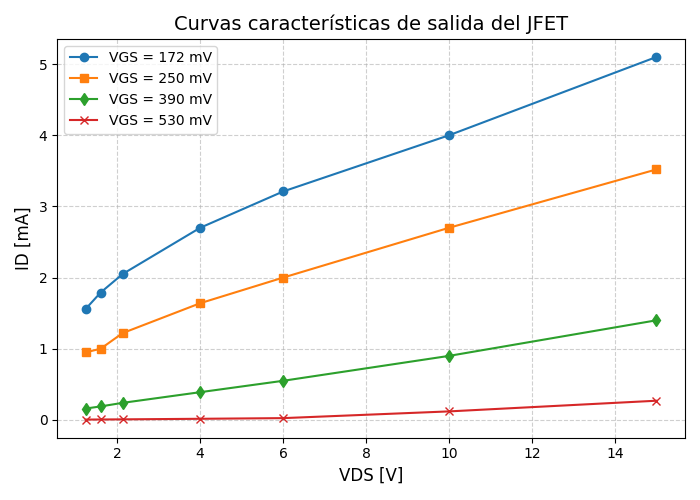
\includegraphics[width=10cm]{./imagenes/grafica3.png}
  
\vspace{0.1cm}

\subsection{Conclusión}
Las curvas medidas muestran el comportamiento esperado del JFET:  $I_D$  disminuye al aumentar la tensión negativa de la compuerta $V_{GS}$.